\chapter{Fission Bank Algorithms}
\label{chap:fission-bank}

\section{Introduction}

We began discussing in \autoref{chap:intro} several aspects of Monte Carlo
simulations that may inhibit them from scaling to large numbers of
processors. One of these aspects is the parallelization of the fission source
iterations that are necessary in an eigenvalue calculation. Traditional parallel
implementations of the fission source iterations have been shown to degrade
parallel efficiency with just tens or hundreds of processors
\cite{physor-hoogenboom-2012}. Thus, in order to scale Monte Carlo eigenvalue
calculations to thousands or millions of processors, a new approach is needed
for parallelizing fission source iterations.

Within each fission source iteration, $N$ source neutrons are simulated and
create $M$ fission sites\footnote{The production of fission sites is weighted
  such that expected value of $M$ is $N$. However, in any given generation, it
  is unlikely that $M=N$ exactly.} that are stored in the fission bank. To
ensure that the neutron population does not grow or shrink exponentially, $N$
source sites for the next generation are randomly sampled from the $M$ fission
bank sites that were stored.

A common requirement in Monte Carlo particle transport codes is that identical
runs should produce identical resuls --- this also applies to parallel
calculations, i.e. a parallel calculation should reproduce the same answers as a
serial calculation. Without reproducibility, it would be difficult to debug or
otherwise verify that modifications to the code do not cause errors. Thus, the
process by which the $N$ source sites are sampled from the $M$ fission bank
sites has to be done in a reproducible manner. Similarly the order of the source
bank sites from one generation to the next should be the same as in a serial
calculation. When an eigenvalue calculation is run in parallel, each process has
its own source bank and fission bank and thus coordination is required between
processes. The use of work scheduling algorithms wherein the mapping of source
sites to processes is non-deterministic make maintaining reproducibility in a
parallel calculation even more challenging.

In \autoref{sec:master-slave}, we present an analysis of a master-slave parallel
algorithm for fission source site sampling and redistribution and elucidate its
limitations. In \autoref{sec:nearest-neighbor}, we introduce a novel algorithm
with a nearest-neighbor communication pattern and present a theoretical analysis
that confirms our intuition that it should scale better than the master-slave
algorithm. Measurements taken within OpenMC to validate the theoretical analysis
are reported in \autoref{sec:fission-bank-validation}. Both algorithms were
implemented in OpenMC to compare their performance and demonstrate scalability
of the nearest-neighbor algorithm on contemporary supercomputers, the results of
which are discussed in \autoref{sec:fission-bank-results}. Finally,
miscellaneous considerations such as load balancing and fault tolerance are
briefly discussed in \autoref{sec:fission-bank-other}.

The material in this chapter largely follows from a paper published in
\emph{Nuclear Science and Engineering} \cite{nse-romano-2012}.

\section{Master-Slave Algorithm}
\label{sec:master-slave}

Monte Carlo particle transport codes commonly implement an SPMD model by having
one master process that controls the scheduling of work while the remaining
processes wait to receive work from the master, process the work, and then send
their results to the master at the end of the simulation. This idea is
illustrated in \autoref{fig:master-slave}.
\begin{figure}[ht!]
  \centering
  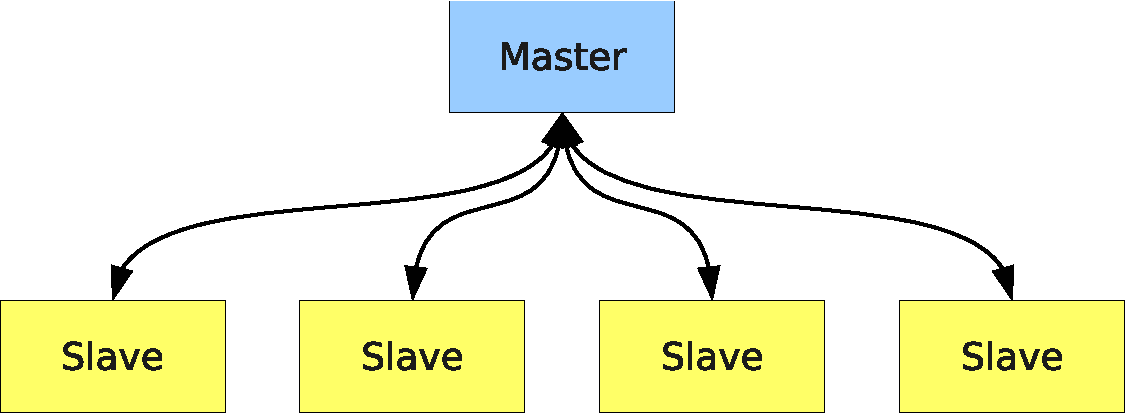
\includegraphics[width=0.8\textwidth]{figures/ch3/master-slave/master-slave.pdf}
  \caption{Typical master-slave algorithm.}
  \label{fig:master-slave}
\end{figure}
The most common parallel algorithm for fission source site sampling and
redistribution also relies on the master process for coordination --- doing so
makes it is easier to achieve reproducibility. In order to guarantee that the
process by which fission sites are randomly sampled does not depend on the
number of processors, the master-slave algorithm is typically implemented in the
following manner \cite{lanl-x5-2008}:
\begin{enumerate}
\item Each slave process \emph{sends} its fission bank sites to the master
  process. With $M$ fission sites in total distributed across the slave
  processes, this step can be completed in $O(M)$ time. Since $E[M] = N$, this
  implies that this step is $O(N)$.
\item The master process sorts or orders the fission sites based on a unique
  identifier. While a naïve sort would require $O(N \log N)$ steps on average,
  Brown outlines a reordering algorithm in \cite{trans-brown-1992} that can
  reduce this to $O(N)$.
\item The master process samples $N$ fission sites from the ordered array of $M$
  sites. This requires a loop over all fission sites and thus, by the same logic
  as before, is $O(N)$.
\item The master process \emph{broadcasts} all the fission sites to the slave
  processes. Since each slave process does not need to keep every source site in
  memory, one could modify the algorithm from a broadcast to a
  \emph{scatter}. However, for practical reasons (e.g. work self-scheduling
  \cite{lanl-brown-2005}), this is normally not done in production Monte Carlo
  codes. This step is also, at best, $O(N)$ as we will see later.
\end{enumerate}
The first and last steps of this algorithm involve communication between the
master and slave processes, whereas the second and third steps require
computation only on the master process. However, each of these steps is $O(N)$
at best. In practice, it is the network communication that becomes prohibitive
and prevents scalability, so we will thus focus our efforts on analyzing the
communication cost.

To estimate the communication cost of the master-slave algorithm, we will
introduce a simple latency-bandwidth model. In this model, we assume that the
time that it takes to send a message between two processes is given by $\alpha +
(dN)\beta$, where $\alpha$ is the time it takes to initiate the communication
(latency), $\beta$ is the transfer time per unit of data (inverse bandwidth),
$N$ is the number of fission sites, and $d$ is the size in bytes of each fission
site.

The first step of the master-slave algorithm is to send $p$ messages to the
master process, each of size $dN/p$ on average. Thus, the total time to send
these messages is
\begin{equation}
  \label{eq:t-send}
  t_{\text{send}} = p\alpha + dN\beta.
\end{equation}
Estimating the time of the broadcast is complicated by the fact that different
MPI implementations may use different algorithms to perform collective
communications. Worse yet, a single implementation may use a different algorithm
depending on how many processes are communicating and the size of the
message. Using multiple algorithms allows one to minimize latency for small
messages and minimize bandwidth for long messages.

We will focus here on the implementation of broadcast in the MPICH2
implementation \cite{ijhpca-mpich-2005}. For short messages, MPICH2 uses a
binomial tree algorithm. In this algorithm, the root process sends the data to
one process in the first step, and then in the subsequent step, both the root
and the other process can send the data to other processes. Thus, it takes a
total of $\lceil \log_2 p \rceil$ steps to complete the communication where
$\lceil x \rceil$ is the smallest integer not less than $x$. The time to
complete the communication is
\begin{equation}
  t_{\text{short}} = \lceil \log_2 p \rceil \left ( \alpha + dN\beta \right ).
\end{equation}
This algorithm works well for short messages since the latency term scales
logarithmically with the number of processes. However, for long messages, an
algorithm that has lower bandwidth has been proposed by Barnett et
al. \cite{sc-barnett-1994} and implemented in MPICH2. Rather than using a
binomial tree, the broadcast is divided into a scatter and an
\emph{allgather}. The time to complete the scatter is $ \log_2 p \: \alpha +
\frac{p-1}{p} N\beta$ using a binomial tree algorithm. The allgather is
performed using a ring algorithm that completes in $(p-1) \alpha + \frac{p-1}{p}
N\beta$. Thus, together the time to complete the broadcast is
\begin{equation}
  \label{eq:t-broadcast}
  t_{\text{long}} = \left ( \log_2 p + p - 1 \right ) \alpha + 2 \frac{p-1}{p}
  dN\beta.
\end{equation}
The fission bank data will generally exceed the threshold for switching from
short to long messages (typically 8 kilobytes), and thus we will use the
equation for long messages. Adding \eqref{eq:t-send} and \eqref{eq:t-broadcast},
we find the total cost of communication for the master-slave algorithm to be
\begin{equation}
  \label{eq:t-master-slave}
  t_{\text{master-slave}} = \left ( \log_2 p + 2p - 1 \right ) \alpha +
  \frac{3p-2}{p} dN\beta.
\end{equation}
For large $N$, it stands to reason that the communication will be
bandwidth-dominated. Based on the bandwidth term in \eqref{eq:t-master-slave},
we see that the combined communication requires $O(N)$ time.

\section{Nearest-Neighbor Algorithm}
\label{sec:nearest-neighbor}

To reduce the amount of communication required in a fission bank synchronization
algorithm, it is desirable to move away from the master-slave algorithm to a
nearest-neighbor algorithm whereby each process communicates only with other
processes that are logically adjacent in the network topology. This concept is
illustrated in \autoref{fig:nearest-neighbor}.
\begin{figure}[ht!]
  \centering
  
\includegraphics[width=0.9\textwidth]{figures/ch3/master-slave/nearest-neighbor.pdf}
  \caption{Nearest-neighbor communication pattern.}
  \label{fig:nearest-neighbor}
\end{figure}

Since the source sites for each fission generation are sampled from the fission
sites banked from the previous generation, it is common in the master-slave
algorithm for a fission site to be banked on one process, sent back to the
master, and finally sent back to the same process as a source site. As a result,
much of the communication inherent in the master-slave algorithm is entirely
unnecessary. By allowing each process to store and sample fission sites locally
and sending sites between processes only as needed, one can cut down on most of
the communication. The proposed algorithm to achieve this works as follows:
\begin{enumerate}
\item An exclusive scan is performed on the number of sites banked, and the
  total number of fission bank sites is broadcasted to all processes. By
  picturing the fission bank as one large array distributed across multiple
  processes, one can see that this step enables each process to determine the
  starting index of fission bank sites in this array. Let us call the starting
  and ending indices on the $i$th process $a_i$ and $b_i$, respectively;
\item Each process samples sites at random from the fission bank using the same
  starting seed. A separate array on each process is created that consists of
  sites that were sampled local to that process, i.e. if the index of the
  sampled site is between $a_i$ and $b_i$, it is set aside;
\item If $a_i$ is less than $iN/p$ where $N$ is the total number of particles
  per generation and $p$ is the number of processors, then send $iN/p - a_i$
  sites to the left adjacent process. Similarly, if $a_i$ is greater than
  $iN/p$, then receive $a_i - iN/p$ from the left adjacent process. This idea is
  applied to the fission bank sites at the end of each process' array as
  well. If $b_i$ is less than $(i+1)N/p$, then receive $(i+1)N/p - b_i$ sites
  from the right adjacent process. If $b_i$ is greater than $(i+1)N/p$, then
  send $b_i - (i+1)N/p$ sites to the right adjacent process. Thus, each process
  sends/receives only two messages under normal circumstances.
\end{enumerate}

The following example illustrates how this algorithm works. Let us suppose we
are simulating $N = 1,000$ particles distributed over four processes. For this
example, it is instructive to look at the state of the fission bank and source
bank at several points in the algorithm:
\begin{enumerate}
\item The beginning of a fission generation where each process has $N/p$ source
  sites;
\item The end of a fission generation where each process has accumulated fission
  sites;
\item After sampling, where each process has some amount of source sites usually
  not equal to $N/p$;
\item After redistribution, where each process again has $N/p$ source sites for
  the next generation.
\end{enumerate}
At the end of each fission generation, each process needs $N/p = 250$ fission
bank sites to continue on the next generation. Suppose that process $p_0$
produces 270 fission banks sites, $p_1$ produces 230, $p_2$ produces 290, and
$p_3$ produces 250. After each process samples from its fission bank sites,
let's assume that $p_0$ has 260 source sites, $p_1$ has 215, $p_2$ has 280, and
$p_3$ has 245. For each process to have the same number of source sites, $p_0$
needs to send its right-most 10 sites to $p_1$, and $p_2$ needs to send its
left-most 25 sites to $p_1$ and its right-most 5 sites to $p_3$. A schematic of
this example is shown in \autoref{fig:nearest-neighbor-example}. The data local
to each process is given a different hatching, and the cross-hatched regions
represent source sites that are communicated between logically adjacent process.
\begin{figure}[ht!]
  \centering
  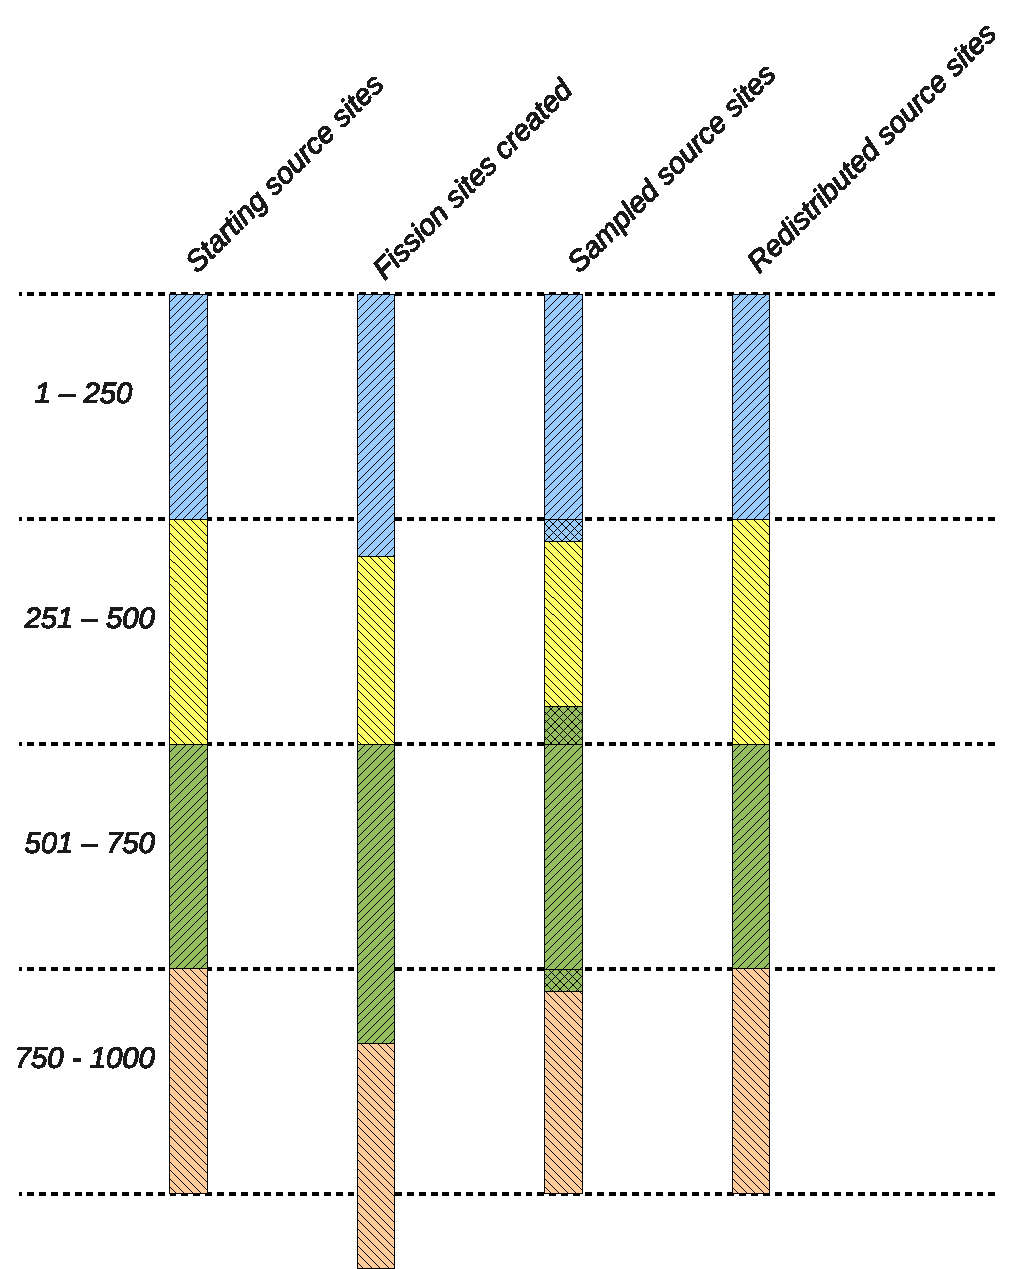
\includegraphics[width=0.9\textwidth]{figures/ch3/algorithm_schematic/nearest-neighbor-example.pdf}
  \caption{Example illustrating nearest-neighbor fission bank algorithm.}
  \label{fig:nearest-neighbor-example}
\end{figure}

Determining the expected communication cost of the nearest-neighbor algorithm is
not trivial due to the fact that the cost will be a function of how many fission
sites are sampled on each process. If each process samples exactly $N/p$ sites,
it would not be necessary to communicate any fission bank sites. However, if any
one process samples more or less than $N/p$ sites, the deviation will result in
communication between logically adjacent processes. To determine the expected
deviation, let us analyze the algorithm based on the fundamentals of the Monte
Carlo process.

The steady-state neutron transport equation for a multiplying medium can be
written in the form of an eigenvalue problem \cite{nukleonik-lieberoth-1968},
\begin{equation}
  \label{eq:NTE}
  S(\mathbf{r})= \frac{1}{k} \int F(\mathbf{r}' \rightarrow
  \mathbf{r})S(\mathbf{r}')\: d\mathbf{r},
\end{equation}
where $\mathbf{r}$ is the spatial coordinates of phase space, $S(\mathbf{r})$ is
the source distribution defined as the expected number of neutrons born from
fission per unit phase-space volume at $\mathbf{r}$, $F( \mathbf{r}' \rightarrow
\mathbf{r})$ is the expected number of neutrons born from fission per unit phase
space volume at $\mathbf{r}$ caused by a neutron at $\mathbf{r}'$, and $k$ is
the fundamental mode eigenvalue.

In a Monte Carlo eigenvalue calculation, the power iteration method is applied
iteratively to obtain stochastic realizations of the source distribution and
estimates of the $k$-eigenvalue. Let us define $\hat{S}^{(m)}$ to be the
realization of the source distribution at fission generation $m$ and
$\hat{\epsilon}^{(m)}$ to be the deviation from the deterministic solution
arising from the stochastic nature of the tracking process. We can write the
stochastic realization in terms of the fundamental source distribution and the
fluctuating component as \cite{ane-brissenden-1986}
\begin{equation}
  \label{eq:source}
  \hat{S}^{(m)}(\mathbf{r})= N S(\mathbf{r}) + \sqrt{N}
  \hat{\epsilon}^{(m)}(\mathbf{r}),
\end{equation}
where $N$ is the number of particle histories per generation. Without loss of
generality, we shall drop the superscript notation indicating the generation as
it is understood that the stochastic realization is at a particular
generation. The expected value of the stochastic source distribution is simply
\begin{equation}
  E \left[ \hat{S}(\mathbf{r})\right] = N S (\mathbf{r})
\end{equation}
since $E \left[ \hat{\epsilon}(\mathbf{r})\right] = 0$. The noise in the source
distribution is due only to $\hat{\epsilon}(\mathbf{r})$ and thus the variance
of the source distribution will be
\begin{equation}
  \text{Var} \left[ \hat{S}(\mathbf{r})\right] = N \text{Var} \left[
    \hat{\epsilon}(\mathbf{r}) \right].
\end{equation}
Lastly, the stochastic and true eigenvalues can be written as integrals over all
phase space of the stochastic and true source distributions, respectively, as
\begin{equation}
  \label{eq:k_to_source}
  \hat{k} = \frac{1}{N} \int \hat{S}(\mathbf{r}) \: d\mathbf{r} \quad \text{and}
  \quad k = \int S(\mathbf{r}) \: d\mathbf{r},
\end{equation}
noting that $S(\mathbf{r})$ is $O(1)$ since the true source distribution is not
a function of $N$ (see Nease et al. \cite{mc-nease-2009} for a thorough
discussion). One should note that the expected value $k$ calculated by Monte
Carlo power iteration (i.e. the method of successive generations) will be biased
from the true fundamental eigenvalue of \eqref{eq:NTE} by $O(1/N)$
\cite{ane-brissenden-1986}, but we will assume henceforth that the number of
particle histories per generation is sufficiently large to neglect this bias.

With this formalism, we now have a framework within which we can determine the
properties of the distribution of expected number of fission sites. The explicit
form of the source distribution can be written as
\begin{equation}
  \hat{S}(\mathbf{r}) = \sum_{i=1}^{M} w_i \delta( \mathbf{r} - \mathbf{r}_i )
\end{equation}
where $\mathbf{r}_i$ is the spatial location of the $i$th fission site, $w_i$
is the statistical weight of the fission site at $\mathbf{r}_i$ (i.e. the weight
of the neutron entering into a fission reaction), and $M$ is the total number of
fission sites. It is clear that the total weight of the fission sites is simply
the integral of the source distribution. Integrating \eqref{eq:source} over all
space, we obtain
\begin{equation}
  \int \hat{S}(\mathbf{r}) \: d\mathbf{r} = N \int S(\mathbf{r}) \: d\mathbf{r}
  + \sqrt{N} \int \hat{\epsilon}(\mathbf{r}) \: d\mathbf{r} .
\end{equation}
Substituting the expressions for the stochastic and true eigenvalues from
\eqref{eq:k_to_source}, we can relate the stochastic eigenvalue to the integral
of the noise component of the source distribution as
\begin{equation}
  N\hat{k} = Nk + \sqrt{N} \int \hat{\epsilon}(\mathbf{r}) \: d\mathbf{r}.
\end{equation}
Since the expected value of $\hat{\epsilon}$ is zero, the expected value of its
integral will also be zero. We thus see that the variance of the integral of the
source distribution, i.e. the variance of the total weight of fission sites
produced, is directly proportional to the variance of the integral of the noise
component. Let us call this term $\sigma^2$ for simplicity:
\begin{equation}
  \text{Var} \left[ \int \hat{S}(\mathbf{r}) \: d\mathbf{r} \right ] = N
  \sigma^2.
\end{equation}
The actual value of $\sigma^2$ will depend on the physical nature of the
problem, whether variance reduction techniques are employed, etc. For instance,
one could surmise that for a highly scattering problem, $\sigma^2$ would be
smaller than for a highly absorbing problem since more collisions will lead to a
more precise estimate of the source distribution. Similarly, using survival
biasing should in theory reduce the value of $\sigma^2$.

Let us now consider the case where the $N$ total histories are divided up evenly
across $p$ processes. Since each process simulates $N/p$ histories, we can write
the source distribution as
\begin{equation}
  \hat{S}_i(\mathbf{r})= \frac{N}{p} S(\mathbf{r}) + \sqrt{\frac{N}{p}}
  \hat{\epsilon}_i(\mathbf{r}) \quad \text{for} \quad i = 1, \dots, p
\end{equation}
Integrating over all space and simplifying, we can obtain an expression for the
eigenvalue on the $i$th process:
\begin{equation}
  \hat{k}_i = k + \sqrt{\frac{p}{N}} \int \hat{\epsilon}_i(\mathbf{r}) \:
  d\mathbf{r}.
\end{equation}
It is easy to show from this expression that the stochastic realization of the
global eigenvalue is merely the average of these local eigenvalues:
\begin{equation}
  \label{eq:average_k_as_sum}
  \hat{k} = \frac{1}{p} \sum_{i=1}^p \hat{k}_i.
\end{equation}
As was mentioned earlier, at the end of each generation one must sample $N$
sites from the $M$ sites that were created. Thus, the source for the next
generation can be seen as the fission source from the current generation divided
by the stochastic realization of the eigenvalue since it is clear from
\eqref{eq:k_to_source} that $\hat{k} = M/N$. Similarly, the number of sites
sampled on each process that will be used for the next generation is
\begin{equation}
  \label{eq:sites_per_node}
  M_i = \frac{1}{\hat{k}} \int \hat{S}_i(\mathbf{r}) \: d\mathbf{r} =
  \frac{N}{p} \frac{\hat{k}_i}{\hat{k}}.
\end{equation}

While we know conceptually that each process will under normal circumstances
send two messages, many of these messages will overlap. Rather than trying to
determine the actual communication cost, we will instead attempt to determine
the maximum amount of data being communicated from one process to another. At
any given generation, the number of fission sites that the $j$th process will
send or receive, $\Lambda_j$, is
\begin{equation}
  \label{eq:Lambda}
  \Lambda_j = \left | \sum_{i=1}^j M_i - \frac{jN}{p} \right |.
\end{equation}
Noting that $jN/p$ is the expected value of the summation, we can write the
expected value of $\Lambda_j$ as the mean absolute deviation of the summation:
\begin{equation}
  E \left [ \Lambda_j \right ] = E \left [ \left | \sum_{i=1}^j M_i -
    \frac{jN}{p} \right | \right ] = \text{MD} \left [ \sum_{i=1}^j M_i \right ]
\end{equation}
where $\text{MD}$ indicates the mean absolute deviation of a random
variable. The mean absolute deviation is an alternative measure of variability.

In order to ascertain any information about the mean deviation of $M_i$, we need
to know the nature of its distribution. Thus far, we have said nothing of the
distributions of the random variables in question. The total number of fission
sites resulting from the tracking of $N$ neutrons can be shown to be normally
distributed via the Central Limit Theorem (provided that $N$ is sufficiently
large) since the fission sites resulting from each neutron are ``sampled'' from
independent, identically-distributed random variables. Thus, $\hat{k}$ and $\int
\hat{S} (\mathbf{r}) \: d\mathbf{r}$ will be normally distributed as will the
individual estimates of these on each process.

Next, we need to know what the distribution of $M_i$ in
\eqref{eq:sites_per_node} is or, equivalently, how $\hat{k}_i / \hat{k}$ is
distributed. The distribution of a ratio of random variables is not easy to
calculate analytically, and it is not guaranteed that the ratio distribution is
normal if the numerator and denominator are normally distributed. For example,
if $X$ is a standard normal distribution and $Y$ is also standard normal
distribution, then the ratio $X/Y$ has the standard Cauchy distribution. The
reader should be reminded that the Cauchy distribution has no defined mean or
variance. That being said, Geary \cite{jrss-geary-1930} has shown that, for the
case of two normal distributions, if the denominator is unlikely to assume
values less than zero, then the ratio distribution is indeed approximately
normal. In our case, $\hat{k}$ absolutely cannot assume a value less than zero,
so we can be reasonably assured that the distribution of $M_i$ will be normal.

For a normal distribution with mean $\mu$ and distribution function $f(x)$, it
can be shown that
\begin{equation}
  \int_{-\infty}^{\infty} f(x) \left | x - \mu \right | \: dx =
  \sqrt{\frac{2}{\pi} \int_{-\infty}^{\infty} f(x) \left ( x - \mu \right )^2 \:
    dx}
\end{equation}
by substituting the probability distribution function of a normal distribution
for $f(x)$, making a change of variables, and integrating both sides. Thus the
mean absolute deviation is $\sqrt{2/\pi}$ times the standard
deviation. Therefore, to evaluate the mean absolute deviation of $M_i$, we need
to first determine its variance. Substituting \eqref{eq:average_k_as_sum} in
\eqref{eq:sites_per_node}, we can rewrite $M_i$ solely in terms of $\hat{k}_1,
\dots, \hat{k}_p$:
\begin{equation}
  M_i = \frac{N \hat{k}_i}{\sum\limits_{j=1}^p \hat{k}_j}.
\end{equation}
Since we know the variance of $\hat{k}_i$, we can use the error propagation law
to determine the variance of $M_i$:
\begin{equation}
  \text{Var} \left [ M_i \right ] = \sum_{j=1}^p \left ( \frac{\partial
    M_i}{\partial \hat{k}_j} \right )^2 \text{Var} \left [ \hat{k}_j \right ] +
  \sum\limits_{j \neq m} \sum\limits_{m=1}^p \left ( \frac{\partial
    M_i}{\partial \hat{k}_j} \right ) \left ( \frac{\partial M_i}{\partial
    \hat{k}_m} \right ) \text{Cov} \left [ \hat{k}_j, \hat{k}_m \right ]
\end{equation}
where the partial derivatives are evaluated at $\hat{k}_j = k$. Since
$\hat{k}_j$ and $\hat{k}_m$ are independent if $j \neq m$, their covariance is
zero and thus the second term cancels out. Evaluating the partial derivatives,
we obtain
\begin{equation}
  \text{Var} \left [ M_i \right ] = \left ( \frac{N(p-1)}{kp^2} \right )^2
  \frac{p\sigma^2}{N} + \sum_{j \neq i} \left ( \frac{-N}{kp^2} \right )^2
  \frac{p\sigma^2}{N} = \frac{N(p-1)}{k^2p^2} \sigma^2.
\end{equation}
Through a similar analysis, one can show that the variance of $\sum_{i=1}^j M_i$
is
\begin{equation}
  \text{Var} \left [ \sum_{i=1}^j M_i \right ] = \frac{Nj(p-j)}{k^2p^2} \sigma^2
\end{equation}
Thus, the expected amount of communication on process $j$, i.e. the mean
absolute deviation of $\sum_{i=1}^j M_i$, is proportional to
\begin{equation}
  \label{eq:comm-cost}
  E \left [ \Lambda_j \right ] = \sqrt{\frac{2Nj(p-j)\sigma^2}{\pi k^2p^2}}.
\end{equation}
Equation \eqref{eq:comm-cost} has all the properties that one would expect based
on intuition:
\begin{itemize}
\item As the number of particle histories increases, the communication cost on
  each process increases as well;
\item If $p=1$, i.e. if the problem is run on only one process, the variance
  will be zero. This reflects the fact that exactly $N$ sites will be sampled if
  there is only one process.
\item For $j=p$, the variance will be zero. Again, this says that when you sum
  the number of sites from each process, you will get exactly $N$ sites.
\end{itemize}
We can determine the process that has the highest communication cost by
differentiating \eqref{eq:comm-cost} with respect to $j$, setting it equal to
zero, and solving for $j$. Doing so yields $j_{\text{max}} =
p/2$. Interestingly, substituting $j = p/2$ in \eqref{eq:comm-cost} indicates
that the maximum communication cost is actually independent of the number of
processes:
\begin{equation}
  \label{eq:nn-cost-max}
  E \left [ \Lambda_{j_{\text{max}}} \right ] = \sqrt{ \frac{N\sigma^2}{2\pi
      k^2}}.
\end{equation}

We can now proceed as before and estimate the communication time using the
latency-bandwidth model. As discussed earlier, each process should send or
receive only two messages, one to each of its neighbors. Since the largest
message will occur on process $j_{\text{max}} = p/2$, we can use
\eqref{eq:nn-cost-max} and \eqref{eq:t-send} to estimate the communication time
for the nearest-neighbor algorithm as
\begin{equation}
  \label{eq:t-nearest-neighbor}
  t_{\text{nearest-neighbor}} = 2\alpha + d\sqrt{\frac{2N\sigma^2}{\pi k^2}} \beta
\end{equation}
To compare the communication time of the two algorithms, we can assume that the
message size is large enough that the communication will be bandwidth
dominated. Dividing \eqref{eq:t-master-slave} by \eqref{eq:t-nearest-neighbor},
we find that
\begin{equation}
  \frac{t_{\text{master-slave}}}{t_{\text{nearest-neighbor}}} = \frac{\left (
    \log_2 p + 2p - 1 \right ) \alpha + \frac{3p-2}{p} dN\beta}{2\alpha +
    d\sqrt{\frac{2N\sigma^2}{\pi k^2}} \beta} \approx \frac{ \left ( 3p - 2
    \right ) k \sqrt{N\pi/2}}{ p\sigma }.
\end{equation}
In the limit of large $p$, this ratio becomes
\begin{equation}
  \label{eq:t-ratio-limit}
  \lim_{p\rightarrow\infty}
  \frac{t_{\text{master-slave}}}{t_{\text{nearest-neighbor}}} =
  \sqrt{\frac{N\pi}{2}} \cdot \frac{3k}{\sigma}.
\end{equation}

We can see from \eqref{eq:t-nearest-neighbor} that the nearest-neighbor
algorithm requires $O(\sqrt{N})$ time instead of $O(N)$ as for the master-slave
algorithm. This should allow the the algorithm to scale to very large numbers of
total processes or particles per generation. In fact, we can show that
arbitrarily good scaling can be achieved. Let $t$ be the time to simulate $N$
particles on $p$ processors. Expressing the network communication time as a
fraction of the time to simulate the particles, we find that:
\begin{equation}
  \frac{t_{\text{nearest-neighbor}}}{t} \propto \frac{\sqrt{N}}{N/p} \propto
  \frac{p}{\sqrt{N}}
\end{equation}
Thus, if we keep $p$ constant and increase $N$, the relative time to complete
network communication will be reduced since the simulation time is proportional
to $N$ and the communication is proportional to $\sqrt{N}$.

\section{Validation of Theoretical Analysis}
\label{sec:fission-bank-validation}

To ensure that any assumptions made in the foregoing analysis are sound, several
test cases using an implementation of the nearest-neighbor fission bank
algorithm in OpenMC were run to provide results that can be compared with the
theoretical analysis. The number of processes and particle histories for each
case are shown in \autoref{tab:cases}.
\begin{table}[ht!]
  \centering
  \caption{Test cases for nearest-neighbor fission bank algorithm.}
  \label{tab:cases}
  \begin{tabular}{ c c c }
    \toprule
    Case & Processes ($p$) & Histories ($N$) \\ 
    \midrule
    1 & 8 & 80,000 \\
    2 & 8 & 160,000 \\
    3 & 16 & 80,000 \\
    4 & 16 & 160,000 \\
    \bottomrule
  \end{tabular}
\end{table}
Each case was run for 10,000 generations and at the end of each run, the
standard deviation of the number of fission bank sites sent to logically
adjacent processes was determined for each process as a proxy for the
communication cost. For Case 1, the data were fit to the following function
(with the same dependence on $j$ and $p$ as in \eqref{eq:comm-cost}) using a
least squares regression:
\begin{equation}
  \label{eq:regression}
  f(j,p,\beta) = \frac{\beta}{p} \sqrt{j(p-j)}.
\end{equation}
The fitting coefficient $\beta$ was then used to predict the expected amount of
communication for the other three cases. \autoref{fig:mean-deviance8} shows the
expected number of fission bank sites sent or received from neighboring
processes, $E \left [ \Lambda_j \right ]$, for Cases 1 and 2 along with the
least squares regression fit based on \eqref{eq:regression} for Case 1 and the
prediction for Case 2. \autoref{fig:mean-deviance16} shows the expected number
of fission bank sites sent or received from neighboring processes for Cases 3
and 4 along with the predicted fits.
\begin{figure}[ht!]
  \centering
  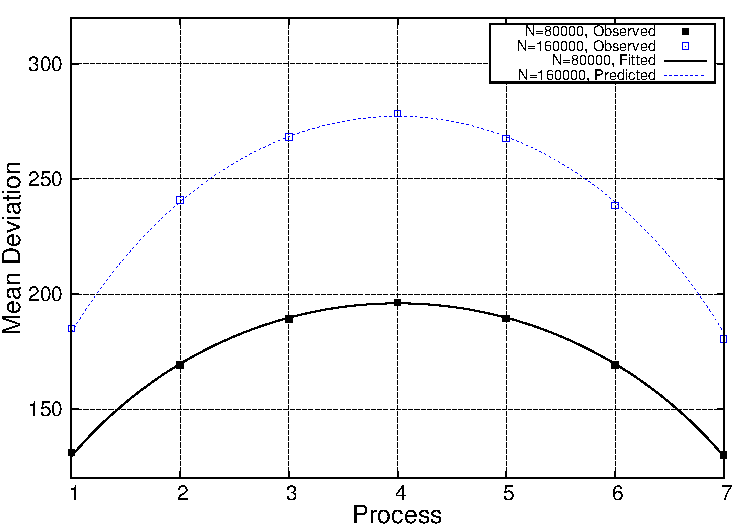
\includegraphics[width=0.75\textwidth]{figures/ch3/mean_deviance/plot8.pdf}
  \caption{Expected number of fission bank sites sent to neighboring processes
    using 8 processes.}
  \label{fig:mean-deviance8}
\end{figure}
\begin{figure}[ht!]
  \centering
  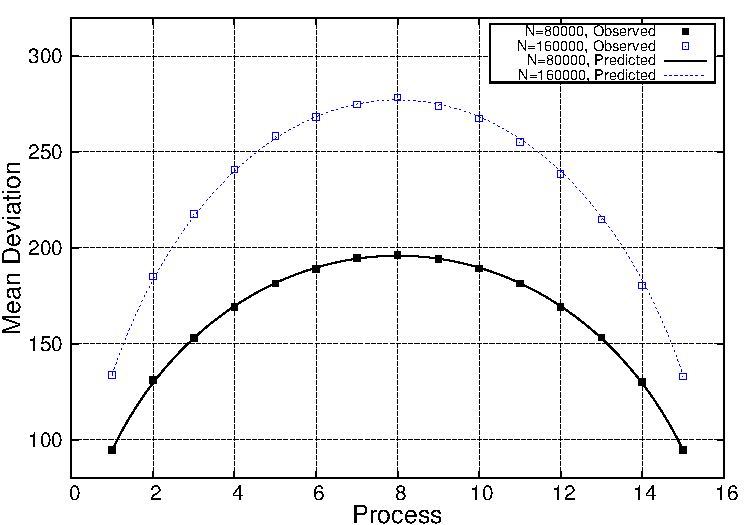
\includegraphics[width=0.75\textwidth]{figures/ch3/mean_deviance/plot16.pdf}
  \caption{Expected number of fission bank sites sent to neighboring processes
    using 16 processes.}
  \label{fig:mean-deviance16}
\end{figure}
A few observations can be made from these figures. Firstly, the data from the
four test cases demonstrates that the foregoing theoretical analysis is indeed
correct. Furthermore, one can observe from these two figures that the maximum
communication does occur for process $j_{\text{max}} = p/2$ and that this
maximum is independent of $p$ as predicted.

It is also instructive to check our assumption that $\sum_{i=1}^j M_i$ is
normally distributed. One way of doing this is through a quantile-quantile (Q-Q)
plot, comparing the observed quantiles of the data with the theoretical
quantiles of the normal distribution. If the data are normally distributed, the
points on the Q-Q plot should lie along a line. \autoref{fig:QQ-plot} shows a
Q-Q plot for the number of fission bank sites sent or received on the first
process for Case 1.
\begin{figure}[ht!]
  \centering
  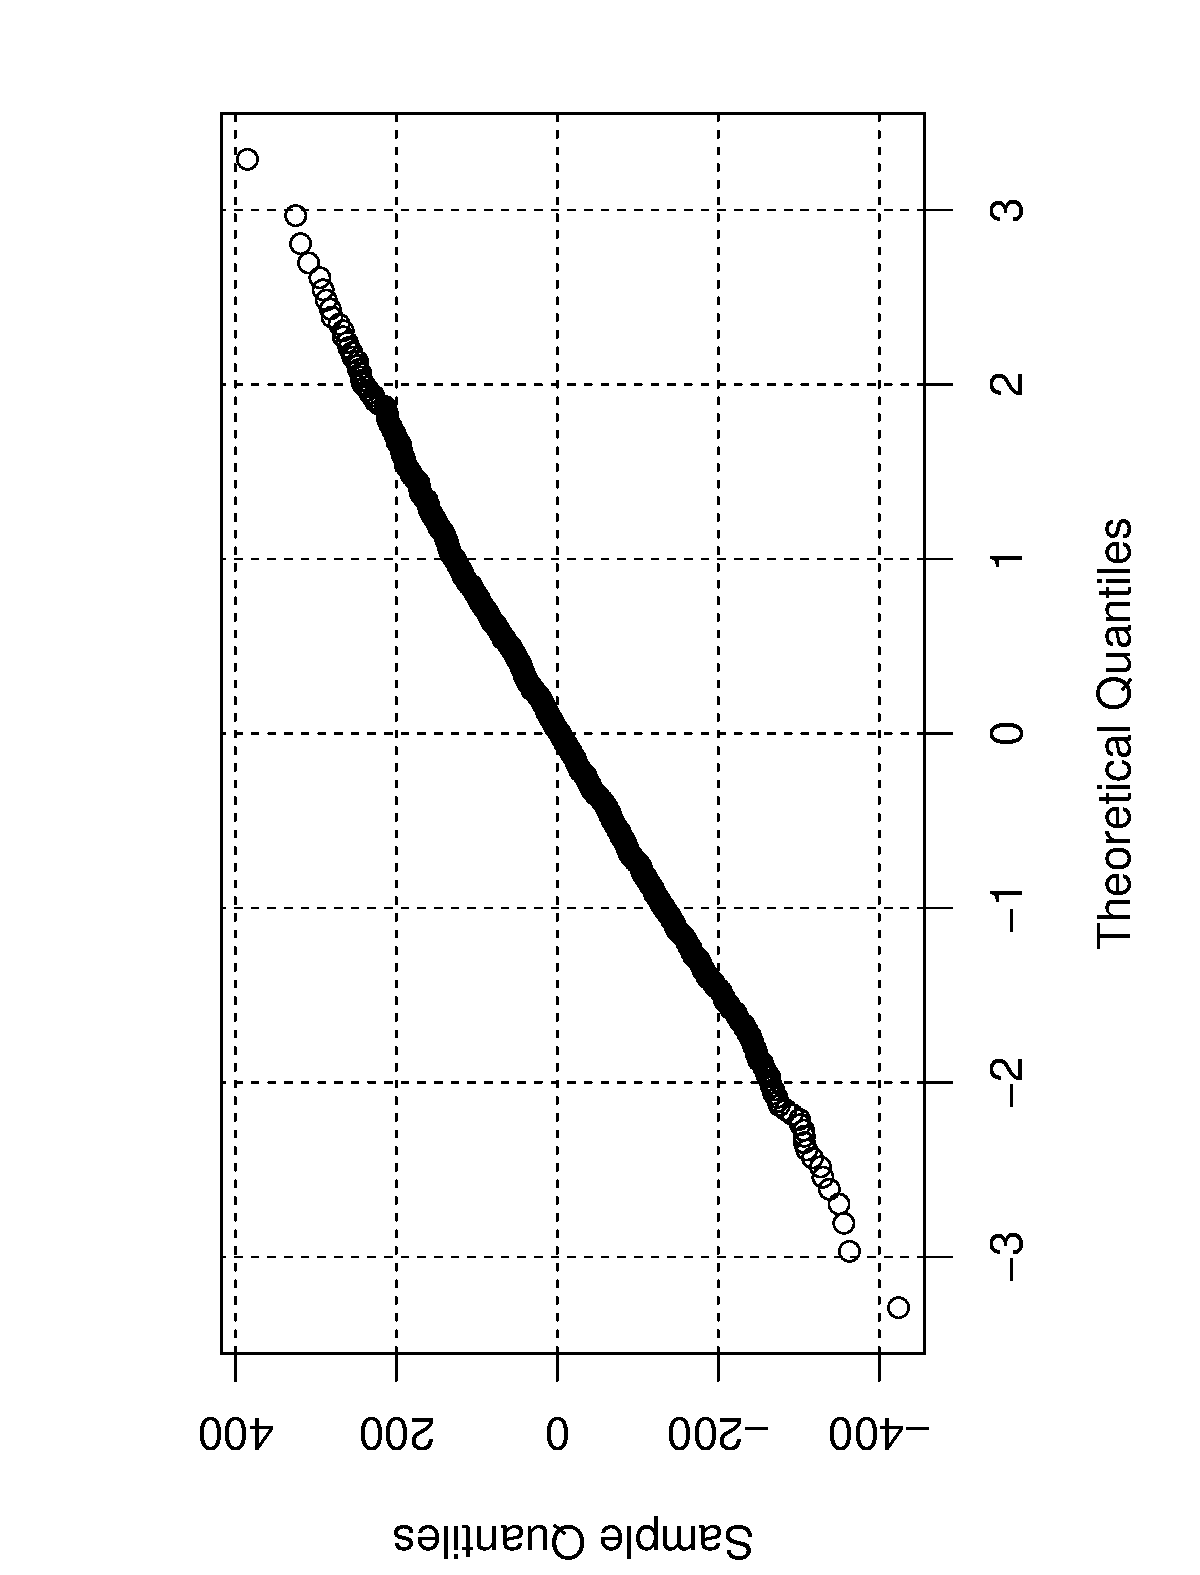
\includegraphics[width=0.75\textwidth,angle=-90]{figures/ch3/QQ_plot/QQplot.pdf}
  \caption{Q-Q plot of $M_1$ for Case 1}
  \label{fig:QQ-plot}
\end{figure}
The data clearly lie along a straight line and thus the data are normally
distributed. This conclusion was also confirmed using the Shapiro-Wilk test for
normality \cite{biometrika-shapiro-1965}.

\section{Results}
\label{sec:fission-bank-results}

\subsection{Communication Time}

In \autoref{sec:nearest-neighbor}, it was shown that the communication cost of
nearest-neighbor algorithm will depend on a parameter $\sigma$ representing the
variance in the number of sites sent between adjacent processes. Thus, while we
can conclude from \eqref{eq:t-ratio-limit} that the nearest-neighbor algorithm
will certainly outperform the master-slave algorithm in the limit of large $p$
and $N$, it is more difficult to make inferences regarding the performance of
the two algorithms for smaller cases.

In order to compare the two algorithms, both were implemented in OpenMC. A
separate simulation using each of the algorithms was run from a single process
up to 88 processes in parallel on a small cluster with an Ethernet network
interconnect. In each case, the number of histories was 40,000 times the number
of processes so that each process simulates the same number of histories. Each
simulation was run for 20 fission generations. \autoref{fig:algorithm-time}
shows the total time spent on fission bank synchronization for the two
algorithms.
\begin{figure}[ht!]
  \centering
  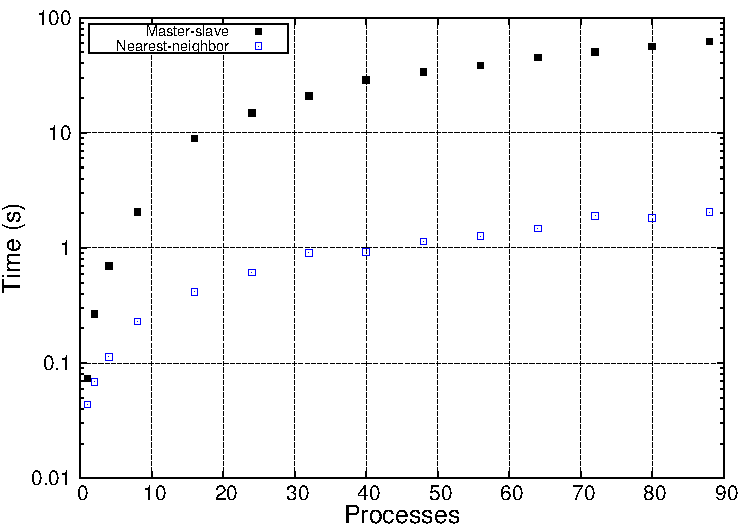
\includegraphics[width=0.75\textwidth]{figures/ch3/algorithm_results/time.pdf}
  \caption{Execution time for fission bank algorithms.}
  \label{fig:algorithm-time}
\end{figure}
We see that the the nearest-neighbor algorithm performs nearly two orders of
magnitude faster than the master-slave algorithm for large $p$ and large $N$. In
these simulations, we have ignored the time spent sampling fission sites and
copying data in memory which may become non-negligible for large $N$. Thus, to
truly demonstrate scalability, simulations with much larger $N$ and $p$ are
needed.

\subsection{Parallel Scaling}

To test parallel scaling, an OpenMC model of the Monte Carlo Performance
Benchmark was simulated on both the Blue Gene/P at the Argonne Leadership
Computing Facility (Intrepid) and the Cray XK6 at the Oak Ridge Leadership
Computing Facility (Jaguar) using the nearest-neighbor fission bank
algorithm. On the Blue Gene/P, up to 163,840 cores were used with 4000 particles
per processor core per generation. On the Cray XK6, up to 131,072 cores were
used with 20,000 particles per processor core per generation. For this study,
the total work per processor was kept constant (weak scaling) rather than the
total amount of work over all processors (strong scaling). \autoref{fig:scaling}
shows the effective number of particles simulated per second as a function of
the number of processors in comparison to the ideal calculation rate (assuming
no communication between fission source iterations). Excellent parallel
efficiency is achieved even above 100,000 processors.
\begin{figure}[ht]
  \centering
  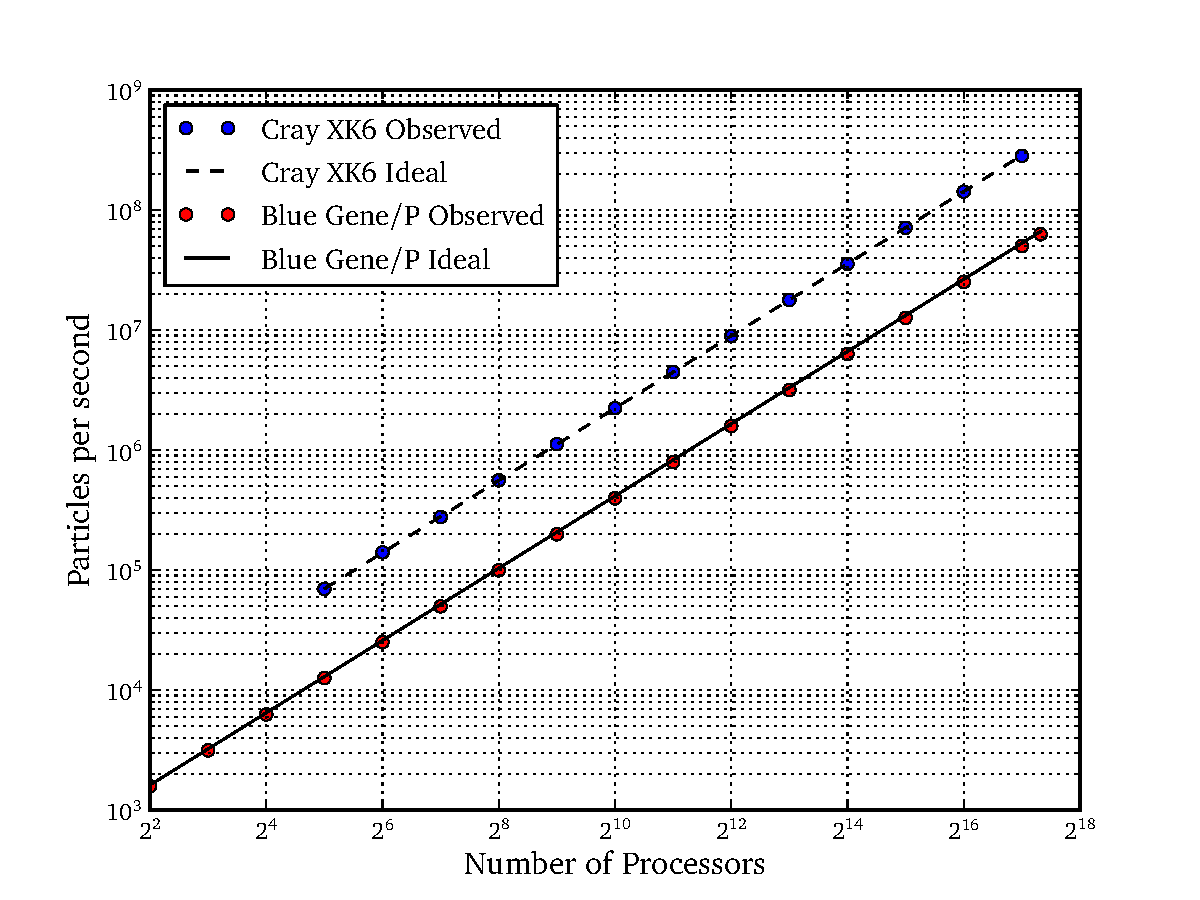
\includegraphics[width=0.9\textwidth]{figures/ch3/scaling/scaling_loglog.pdf}
  \caption{Parallel scaling for the Monte Carlo Performance Benchmark on the
    Cray XK6 (Jaguar) and Blue Gene/P (Intrepid) supercomputers.}
  \label{fig:scaling}
\end{figure}

A few notes should be made regarding the achieved scaling shown in
\autoref{fig:scaling}. First, it was necessary to use non-blocking communication
semantics rather than blocking communication; when blocking communication was
attempted, the scaling behavior was observed to be much worse. Additionally, it
was necessary to turn off the calculation of Shannon entropy during the
simulations. In OpenMC, the number of mesh cells used for the Shannon entropy
mesh grows linearly with the number of particles per generation. At the end of
the fission generation, the number of source sites in each mesh cell has to be
reduced from all processes before being used in \eqref{eq:shannon-entropy}. As
such, in a series of weak scaling runs, the communication associated with
calculating Shannon entropy would grow linearly with the number of processors
--- turning off the calculation of Shannon entropy circumvents this. Another
simple solution would be to fix the size of the Shannon entropy mesh
irrespective of the number of particles per generation.

\section{Other Considerations}
\label{sec:fission-bank-other}

\subsection{Load Balancing}

One important requirement for a parallel Monte Carlo calculation is proper
load-balancing, i.e. it is undesirable to have a process sitting idle with no
work to do while other processes are still busy working. This is especially the
case when the hardware architecture is heterogeneous (having different types of
processors in a single cluster). In the master-slave algorithm, work
self-scheduling is achieved by having each slave process request small batches
of work from the master, and as each batch is completed, the slave may request
more work. By breaking up the problem into smaller batches, this ensures that in
a single source iteration, a processor that is twice as fast as another
processor will also be assigned twice as many histories to compute, and thus all
processors should finish their work at approximately the same time.

The nearest-neighbor algorithm unfortunately precludes the use of the
aforementioned self-scheduling algorithm since an important aspect of the
algorithm is to assign particle histories sequentially to the processes to
preserve their order. It should be noted that if one did not care to preserve
reproducibility in a calculation, the self-scheduling scheme could easily be
applied for load-balancing with the nearest-neighbor fission bank algorithm.

The results in \autoref{fig:scaling} demonstrate that the lack of a load
balancing mechanism does not degrade parallel efficiency when used on a
homogeneous cluster. Previous studies using MCNP on a homogeneous Linux cluster
have shown a 5-10\% loss in parallel efficiency when not using any sort of load
balancing \cite{lanl-brown-2005}.

It is also possible to employ a basic means of load balancing for heterogeneous
architectures using in the nearest-neighbor algorithm by ``tuning'' the
algorithm to the specific characteristics of the cluster. If one were to measure
the performance of each type of processor on the cluster in terms of particles
processed per second, the number of histories on each processor could be
adjusted accordingly instead of merely distributing particles uniformly ($N/p$
on each processor).

\subsection{Fault Tolerance}

For petascale and future exascale architectures, it is desirable to have some
means of fault tolerance to ensure that not all results are lost in the event of
a hardware failure. In current Monte Carlo codes, this can be achieved by having
all processes periodically rendezvous and collectively dump data to a file that
can be used to restart the run. While providing insurance against lost
simulation time, performing fault tolerance this way unfortunately degrades
parallel performance since it entails collective communication between all
processors. Notwithstanding, the algorithm we have presented here does not
inhibit the use of fault tolerance in this manner.

\section{Conclusions}
\label{sec:conclusions}

In this chapter, we presented a new algorithm for parallelizing the source
iterations in a Monte Carlo criticality calculation. This algorithm takes
advantage of the fact that many of the fission sites produced on one processor
can be used as source sites on that same processor --- in doing so, it avoids
unnecessary communication between processors.

Analysis of the algorithm shows that it should outperform existing algorithms
for fission bank synchronization and that furthermore, the performance gap
increases for an increasing number of histories or processors. Test results on
the OpenMC Monte Carlo code confirm this finding. The analysis also shows that
the maximum amount of communication in the algorithm is independent of the
number of processors and instead will depend on the number of histories per
generation and the physical characteristics of the problem at hand. Again,
testing within OpenMC confirms this prediction. Finally, a scaling study was
performed on the Titan and Intrepid supercomputers and demonstrated perfect
scaling with over 100,000 processor cores using the nearest-neighbor algorithm.

The reader should keep in mind that while the algorithm presented here will
significantly improve the time necessary to sample and distribute fission sites
between generations, it has no effect on the actual transport simulation of
particles moving through a material medium. Thus, it will not improve smaller
simulations that would typically run on a workstation. However, for large
simulations that necessitate the use of a large cluster or supercomputer to
complete in a reasonable amount of time, this novel algorithm will improve the
parallel efficiency and is an important step in achieving scalability up to
thousands or millions of processors.

One potential shortcoming of the present algorithm is that it precludes the use
of load balancing via existing algorithms for heterogeneous computer
architectures. A basic method to provide load balancing in such situations based
on ``tuning'' the algorithm was suggested, although it has not yet been tested.
